\documentclass{article}

% if you need to pass options to natbib, use, e.g.:
%     \PassOptionsToPackage{numbers, compress}{natbib}
% before loading neurips_2018

% ready for submission
% \usepackage{neurips_2018}

% to compile a preprint version, e.g., for submission to arXiv, add add the
% [preprint] option:
%     \usepackage[preprint]{neurips_2018}

% to compile a camera-ready version, add the [final] option, e.g.:
\usepackage[preprint]{nips_2018}

% to avoid loading the natbib package, add option nonatbib:
%     \usepackage[nonatbib]{neurips_2018}

\usepackage[utf8]{inputenc} % allow utf-8 input
\usepackage[T1]{fontenc}    % use 8-bit T1 fonts
\usepackage{hyperref}       % hyperlinks
\usepackage{url}            % simple URL typesetting
\usepackage{booktabs}       % professional-quality tables
\usepackage{amsfonts}       % blackboard math symbols
\usepackage{nicefrac}       % compact symbols for 1/2, etc.
\usepackage{microtype}      % microtypography
\usepackage{amsmath}
\usepackage{graphicx}
\usepackage{caption}
\usepackage{subcaption}

\title{Full Stack Salary Prediction: Find and Predict Resources for Low-Income Salaries}

% The \author macro works with any number of authors. There are two commands
% used to separate the names and addresses of multiple authors: \And and \AND.
%
% Using \And between authors leaves it to LaTeX to determine where to break the
% lines. Using \AND forces a line break at that point. So, if LaTeX puts 3 of 4
% authors names on the first line, and the last on the second line, try using
% \AND instead of \And before the third author name.

\author{%
  Raghavendra P. Koppula \\
  Department of Computer Science\\
  UNC Chapel Hill\\
  \texttt{rpranith@live.unc.edu} \\
  \And
  Mazin Shaaeldin \\
  Department of Computer Science\\
  UNC Chapel Hill\\
  \texttt{mazins@live.unc.edu} \\
  \And
  Michael Alcorn \\
  Department of Computer Science\\
  UNC Chapel Hill\\
  \texttt{malcorn@live.unc.edu} \\
}

\begin{document}
% \nipsfinalcopy is no longer used
\maketitle

\section{Introduction}

This paper uses multiple datasets and methodologies to build a recommendation pipeline for predicting income and economic status. This is a full-stack process of the income lifecycle: from salary prediction to finding job fit.

The primary question we explore is what are the factors that improve and maximize the probability for an individual to increase their income? This question requires new and novel ways to model and predict based on temporal datasets. We explore new ways to model this question mathematically while continuing to explore traditional machine learning (ML) methods and comparing these methods. We define economic well-being, also referred to as “economic status” or “well-offness” as the ability of having a better status than at a previous state, that is $s_{i+1} > s_i$ where $s$ represents the economic status and $i$ represents a temporal metric.

There are 3 major components of the project. First was to find/develop a dataset that was a time-series of income data along with analyzing this data is a precise and mathematical way. The second was to use this new methodology/model and compare it across multiple traditional ML techniques, to see whether our model performed better or worse. Finally, the third component was to build a pipeline that uses the classification and analysis of the features that performed best to build a recommendation pipeline for jobs, resources, and general financial advice. 


\subsection{Salary Classification through Census Data}

We will begin by outlining our specific datasets. First, we are using a dataset from University of Calofironia Irvine's (UCI) website titled “Adult Data Set.” This is an extraction that was done by Barry Becker on 1994 Census data. This was the most recent census dataset were were able to find that was mostly processed and cleaned. It was extracted on the following conditions: (AAGE>16) \& (AGI>100) \& (AFNLWGT>1) \& (HRSWK>0). The target variable was a boolean indicator that was coded as 1 for salaries $\ge 50$k and 0 for $\le 50$k. 

We began by pre-processing our data. We noticed there is a skew in our data as the capital gain and capital loss columns are high, so we cube root it. In order for our classification model to work, our data must be in int/float format. Hence we used LabelEncoder from scikit-learn to encode our data. We used Standard Scaler from the same library to scale our data such that the mean is 0 and standard deviation is 1 to allow for our model to learn better.


\subsection{Kiva Loan / Lower Income Analysis}

This dataset is from Kiva, a non-profit organization that provides loans to people around the developing world. The target variable was loan funded amount, which is a real value that is the amount of loan provided to a family. This dataset was chosen as an extension of the original proposal to find resources for lower income family. Therefore, this dataset can provide us with features that may help to gather a larger loan, which maybe financially beneficial to these families.

\subsection{Glassdoor Job Listings}

This data is a scraping of the Glassdoor job listings website, where the target variable is an expected salary outlook for each job description. The purpose of this dataset is to complete the full-stack nature of the income lifecycle, whereby matching people from the previous two datasets with jobs with this dataset completes this pipeline. 

\section{Related Works}

Since this paper focuses on an application based method, research into specifically income classification was pretty standardized. This is important, but research relating to improvements and novel ideas on finding unique factors about features that help improve income was scarce. However, multiple studies have looked into using various unique machine learning techniques to improve income/socioeconomic status classification, clustering, and regression tasks. 

Starting with papers that use similar datasets and standard models, Wang (2022) \cite{wang} used the same UCI dataset and tested multiple ML methods on the data, and found that k-nn and random forrest classifiers were the best regarding accuracy of the model. Chakrabarty, et al. (2018) \cite{chakrabarty} also used the UCI dataset and found that Gradient Boosting Classifier (GBC) performed the best compared to the standard ML algorithms. Lazar (2004) \cite{lazar} found that SVM and PCA reduced the dimensions of the data and decreased computational time by 60\%, however there was a tradeoff in classifier accuracy.

Sharaf, et al. (2022) \cite{sharaf} surveyed many recommendation system in the financial service space, finding that there are primarily two types of recommendation algorithms: collaborative filtering and content-based filtering. The former focuses on data sources and filters based on various sources that is memory based, while the latter focuses on finding similarity to user preferences. This paper and project leans more towards the content-based filtering methodology because of the individual predictive nature of the project. Based on an individuals features, the project aims to predict their income, which therefore requires a individual focused algorithm. 

Musto, et al. (2015) \cite{musto} developed a novel case-based recommendation system that seeks to diversify and produce investment portfolio's of individual investors and maximize their gains. The main idea of the paper included pipeline that was recycled for new problems, defined as custom data structure of the form $<u_i, p_i, f_i>$, where $u_i$ represents a feature vector of 8 values regarding the portfolio, $p_i$ is the distribution of the portfolio assets and $f_i$ is the yield obtained the portfolio. This datastructure is fed through a case-base lifecycle pipeline where using the k-nn algorithm, similar cases are found and the portfolio's that are the most similar are ranked and used to update the current portfolio. They found that their system outperformed human investors in testing in short-term and long-term realizations. 

Ayasse, et al. (2016) \cite{ayasse} use Markov chains to predict the probabilities of each state where achieving the american dream is possible. Mathematically, this is described as the $\mathbb{P}(\text{child}Q_j | \text{parent}Q_i)$, whereby $s$ is the state, $Q_j$ is the quantitle of wealth/income/school-spending of the child, and $Q_i$ is the quantile of the parent. Thus, it is asking for the probability that $j > i$, and this can be mapped on to a transition matrix and the markov property can be used to calculate probabilities for each state.

The most applicable paper to the project is Barratt, et al. (2022) \cite{barratt} by where they use Markov chains to fit feature matrices to find applications to real world data. They do this by modelling state changes as 
$$\mathbb{P}_{\theta}(y_{t+1} = j | y_t = i) = P_{ij}$$
meaning that transitioning from state $j$ to $i$ can be modeled as a probability using a transition matrix $P$, where $P_{ij}$ represents the probability of transitioning from state $i$ to $j$. They use a logisitic preditor to model the probability distribution and maximize the log-likelihood of the above distribution. They then fit this model to two real world data-sets in baseball and stock predictions. 

Clearly, many different methodologies exist using various techniques to build classification systems for salary and income prediction. This paper will continue to add to this literature using traditional ML techniques while adding to novel methods such as the Markov chain for feature-dependent data. 

\section{Methods}

\subsection{Mathematical Modelling using Additive Markov chains}

Traditional markov chains have the assumption of the markov property, which states that the state $t+1$ only depends on the previous state $t$ and therefore is independent of any $t-1, t-2, ..., 1$ states. However, this is not necessarily true in many real world applications. Specifically for salary and income predictions, the monthly status of an individual's income may have a large effect on the future state. Further, a specific feature such as if the person holds a large balance / credit-card debt in their previous montly status can impact future classification.
The probability distribution that the question asks is
$$\mathbb{P}_{\theta}(y_{t+1} = j | y_t = i_{t}, y_{t-1} = i_{t-1}, y_{t-2} = i_{t-2}, ..., y_{t-m} = i_{t-m})$$
Concretly, this is like finding the probability that a person will move to a middle-class income conditioned on that the last 4 monthly income states were low-income, middle-income, low-income, low-income. Thus, we find the parameters $\theta$ that maximizes this probability.  This is just
$$\underset{\theta}{\operatorname{argmax}} \prod_{i=1}^N \mathbb{P}_{\theta}(y_{t+1} = j | y_t = i_{t}, y_{t-1} = i_{t-1}, y_{t-2} = i_{t-2}, ..., y_{t-m} = i_{t-m})$$
where $m$ is the number of states you want to go back to. 

This is an additional step in the direction of using markov chain to model state based movements. The data required to apply this is of time-series in nature, which is complicated and difficult to obtain. However, there are various applications if such data is availabile: finding parameters that maximize the change from one income class to another, sports state decision making, financial stock trading, etc. The next steps for this model will be explained in the future plans section.

\subsection{Mathematical Modelling using Traditional Methods}
Traditional machine learning methods use the probability distribution 
$$\underset{\theta}{\operatorname{argmax}} \prod_{i=1}^N \mathbb{P}_\theta(y_i \mid x_i)$$
We then simplify maximize the probability of prediting $y_i$ conditioned on $x_i$ by finding the parameters $\theta$. Both classification and regression methodology use the same principle as above. 

\paragraph{Linear Regression}
We use Linear Regression in the Kiva dataset, whereby loan amounts are a continous variable with various factors. Some decisions to we made to simplify and make the model better were to drop missing rows due to the limited nature of them and standardize the data for $\mu = 0$ and $\sigma^2 = 1$. We used the standard mean squared error (MSE). Some additions we did not include were a regularizer. A regularizer is most probably required due to the large nature of the dataset, however it was not implemented in this version. 

\paragraph{Multinomial Naive Bayes} was used in the Glassdoor job data, whereby text features were used to predict the category of a high or low paying job. Then the probabilistic model is
$$\mathbb{P}(C = c | W) = p(c) \prod_{i=1}^{n}p(w_i | c)$$
where $C$ is a binary class with 0 represents less than the 50th percentile in salary, and 1 the opposite, $W$ is a string of words or a single word, and $p(c)$ is the prior probability of the $c$ class. Then, we maximize the log likelihood of the function, which can represented as
$$c = \underset{i \in {0,1}}{\operatorname{argmax}} |\mathbb{P}(C_i | W)|$$
This will require the use of bag-of-words representation for the text data to be processed as a vector in the model, along with multiple nlp steps to clean the word data. 

\paragraph{Logistic Regression, K-nn, and Gaussian Naive Bayes} were used to classify the UCI dataset. These models are pretty standard, and required less mathematical tuning. The main concepts to use are to perform cross-validation to find the best $k$, and to remove any feature variables that are discrete for the gaussian naive bayes (GNB) classifier as it inherently assumes normal distribution for each feature. 

\section{Preliminary Results}

\subsection{UCI Classification}

Looking at our conducted experiments thus far, we have three sets of results from each respective experiment. Beginning with our classification task, we utilized the “Adult Data Set” to classify salaries either above or below fifty thousand U.S. dollars. We trained the model using 3 classifiers: gaussian naive bayes, logistic regression, and k-neighbors with the number of neighbors set to five. Figure 1 shows the results of our findings for each classifier.

\begin{figure}
  \centering
  \begin{subfigure}[b]{0.5\textwidth}
      \centering
      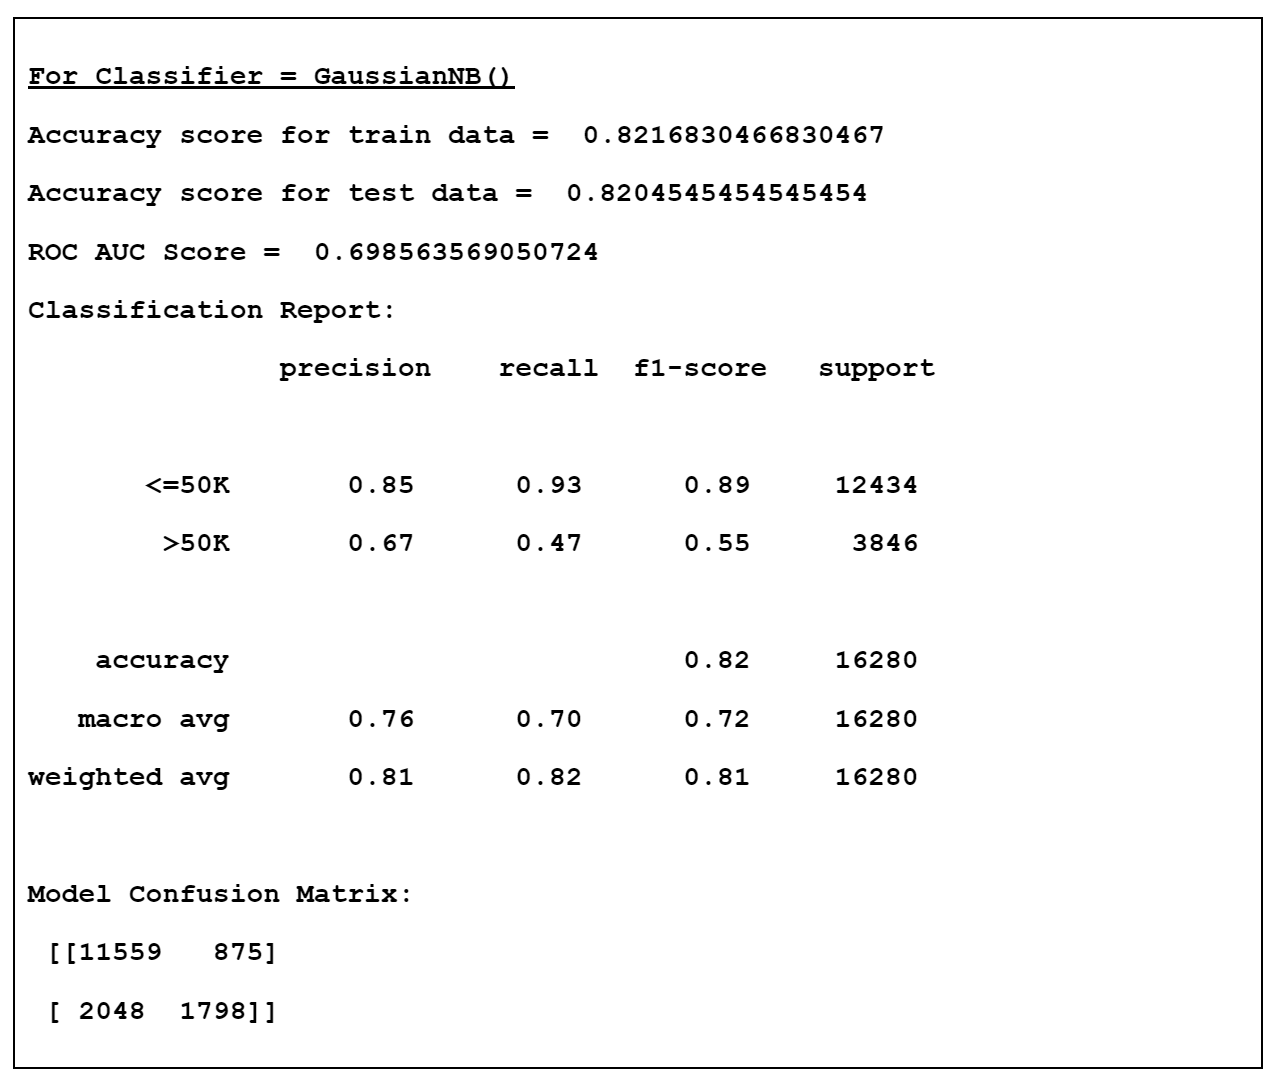
\includegraphics[width=\textwidth]{gnb_uci.PNG}
      \caption{Gaussian Naive Bayes}
      \label{fig:y equals x}
  \end{subfigure}
  \hfill
  \begin{subfigure}[b]{0.5\textwidth}
      \centering
      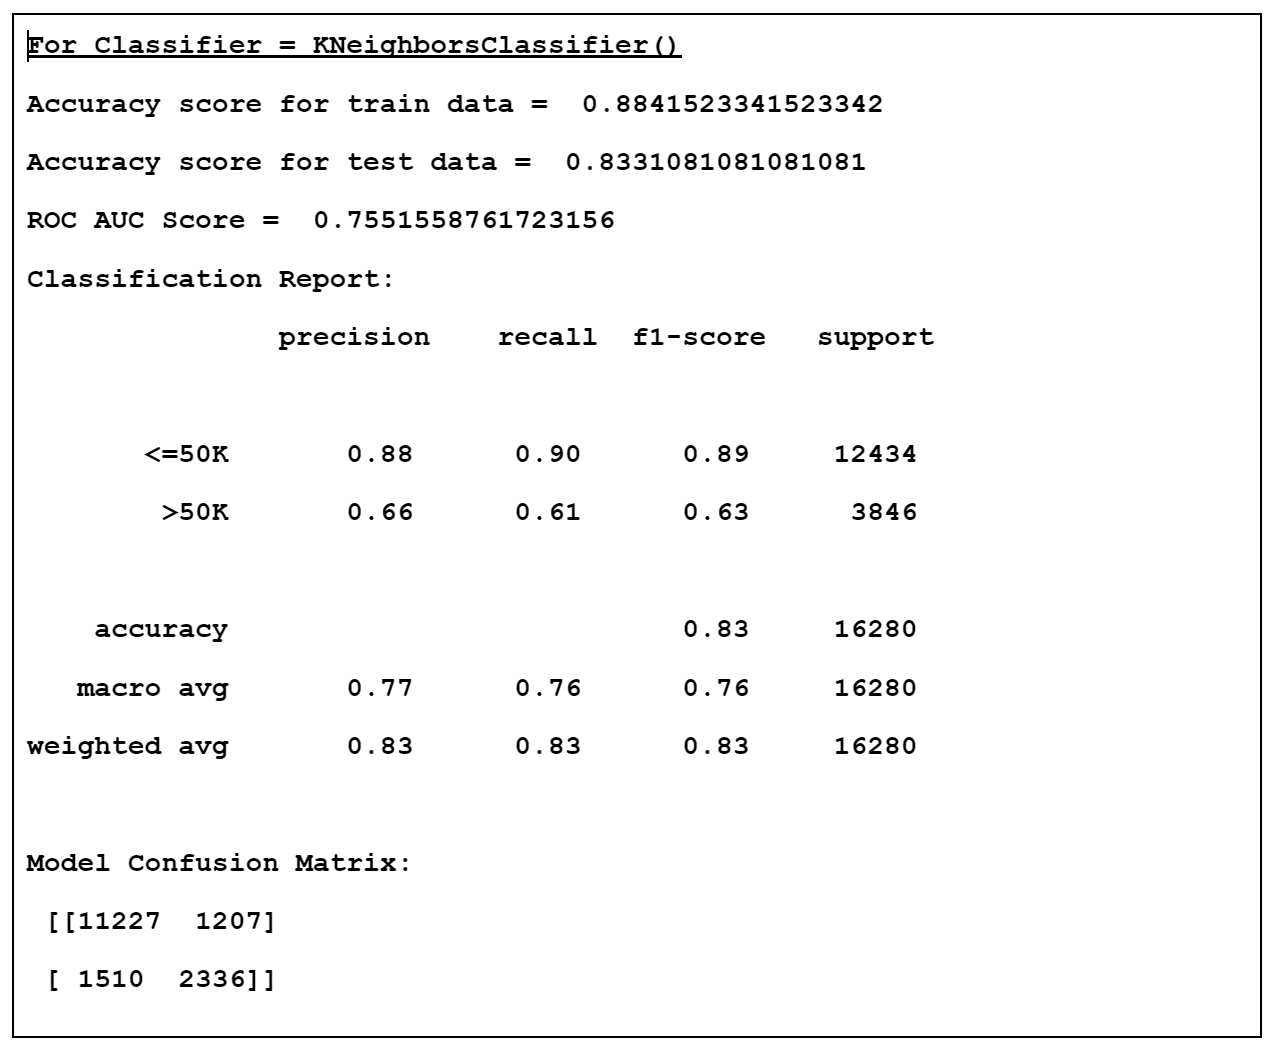
\includegraphics[width=\textwidth]{knn_uci.PNG}
      \caption{K-nn where $k = 5$}
      \label{fig:three sin x}
  \end{subfigure}
  \hfill
  \begin{subfigure}[b]{0.5\textwidth}
      \centering
      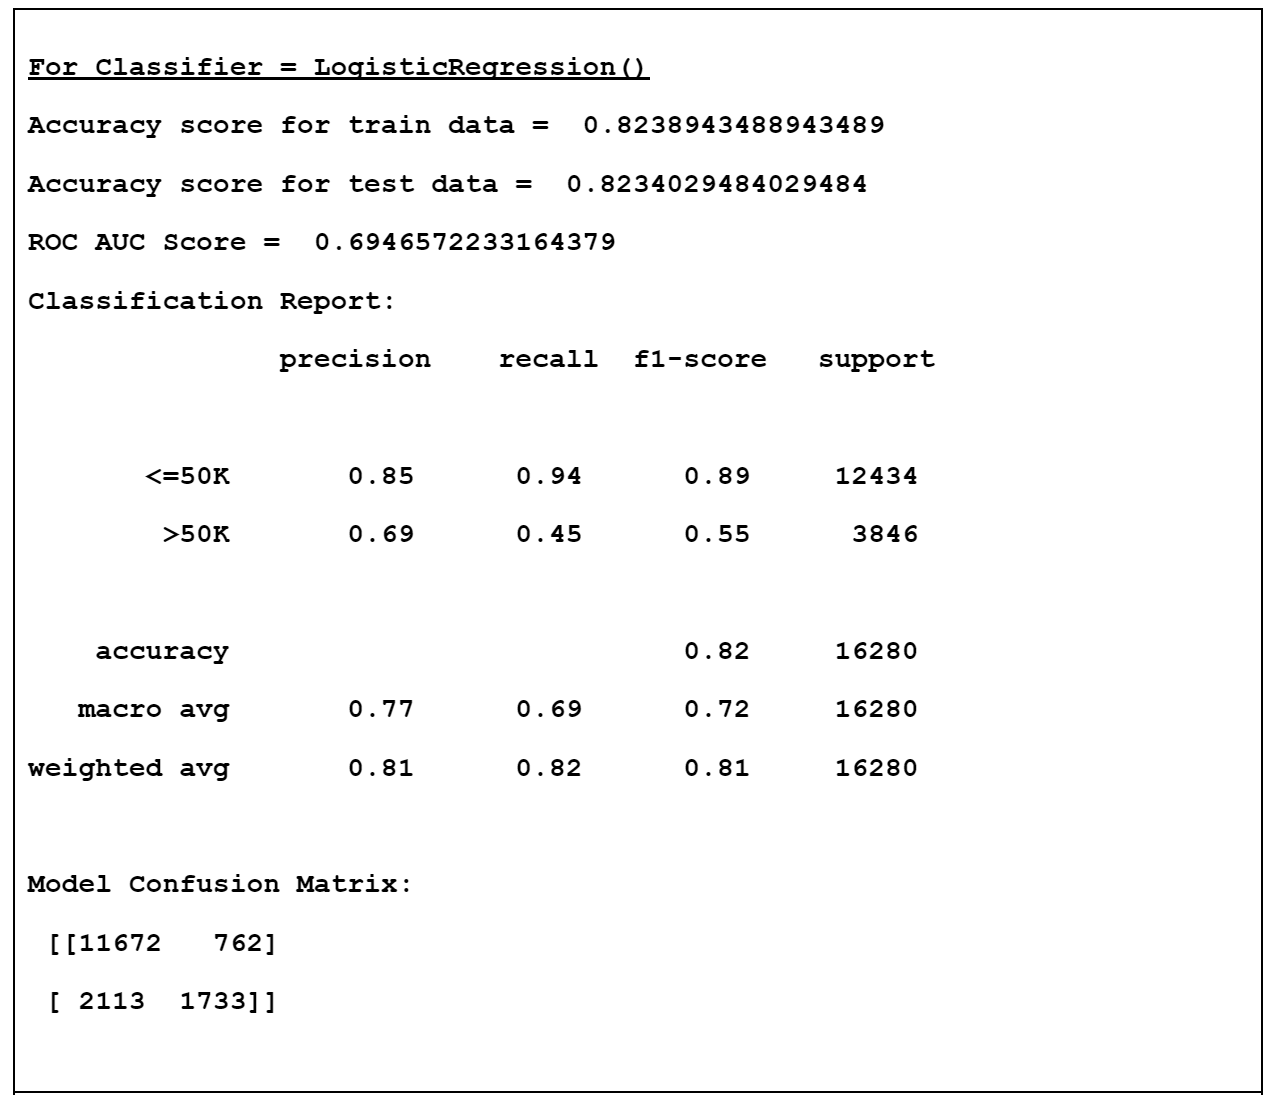
\includegraphics[width=\textwidth]{lgr_uci.PNG}
      \caption{Logistic Regression}
      \label{fig:five over x}
  \end{subfigure}
     \caption{Classification results on UCI dataset}
     \label{fig:three graphs}
\end{figure}

Upon looking at these results, we can see that our accuracy for training and test data when using the Gaussian Naive Bayes classifier and Logistic Regression is around 82\%. For the K-Neighbors classifier when using 5 neighbors, the training accuracy is about 88\% and the test accuracy is around 83\%. These results would lead us to believe that K-Neighbors is the most effective classifier for predicting salary above or below 50k, but we must check the ROC AUC score as well for each classifier. The ROC AUC for Gaussian Naive Bayes and Logistic Regression are both 70\% while the ROC AUC score for K-Neighbors is around 75\%. We can confirm that the K-Neighbors classifier is the most effective classifier for our data set. 

\subsection{Kiva Loan Regression}

Moving on to our work analyzing income and loan correlation, we wanted to see what parameters affected a person's received loan amount. The features that affected the loan amount the most were the country, lender\_count, location\_type, and conflicts\_total. We were surprised to see that the use of the loan and the activity was close to 0 for weighting. We evaluated the model using mean squared error and got an MSE value of 1156.44 and an R square value for the normal equation method of: 0.72. 

One challenge with Linear Regression is that the data is heterogeneous, meaning that the features are very independent from each other and the correlation between the features is low. Further, the highly correlated features are variables like country, which requires a clever way to encode. These decisions need to be made and implemented to improve the model.

\subsection{Glasdoor Job Listings}

Finally, the goal for our third experiment was to process unstructured data (job description) and predict salary using NLP. After lots of pre-processing such as removing punctuation, newline characters, and tokenizing, we had to decide on a normalization technique that would fit the dataset best. Using a bag of words representation and multinomial bayes classifier, we received 85\% accuracy and an ROC AUC score of around 86\%.

\section{Future Plans}

Looking towards the future, we have these actionable items to complete in order to finalize our project.

There exists a dataset called the Current Population Survey (CPS) which contains temporal data on individual household income over multiple months that we found only recenlty. This dataset provides the exact data required for the original proposal, and the methodology of implementing Markov chains would give us the exact final product we are looking for: the factors that maximize a state transition of income. We plan to explore this dataset and build our final project around this if the experiments we conduct work over the next week. If over the next week we find that there are challenges, we plan to continue to explore traditional ML methods and improve our existing models.

Then we want to use cross-validation to detect and prevent overfitting. Avenues that we may take in using cross-validation include hold-out, K-fold, and leave-one-out cross validation. In this, we hope to test multiple variations for regularization terms, the best $k$, and other hyperparameter searches. We are hoping to complete this in the next week in order to move on to the next step. 

We hope to merge each of our individual findings into a streamlined output. Right now, we have worked on predicting salary through three different ways: Classification, linear regression, and job description. On top of that, we have looked at which factors affect loan receival. We must determine the intersection of each and value the efficacy of individual methods over another. We understand that this step will take a lot of analysis and collaboration, so we will devote ourselves around a week and half to complete this task. Once we do that, we plan to move onto our next step. 

We also want to explore and implement a neural network to predict salary. Right now, our personal knowledge in implementing neural networks is quite limited and we plan to research implementations while we complete our previous two steps. We believe that implementation of the neural network will take around a week. 

Then we want to wrap up our findings and write a final report. We are hoping that this will take us one more week of collaboration. This would leave our final completion date during the last week of classes starting on April 24th. 


\bibliographystyle{plain}
\bibliography{ref}

\end{document}
